\chapter{Exercise 03}
\extitle{ColorFilter}
\turnindir{ex03}
\exnumber{03}
\exfiles{ColorFilter.py}
\exforbidden{None}
\makeheaderfilesforbidden


% ================================= %
\section*{Objective}
% --------------------------------- %
Manipulation of loaded image via numpy arrays, broadcasting.

% ================================= %
\section*{Instructions}
% --------------------------------- %
You have to develop a tool that can apply a variety of color filters on images.\\
\\
For this exercise, the authorized functions and operators are specified for each methods.
You are not allowed to use anything else.\\
\\
Write a class named \texttt{ColorFilter} with 6 methods with the following exact signatures:

\begin{minted}[bgcolor=darcula-back,formatcom=\color{lightgrey},fontsize=\scriptsize]{python}
def invert(self, array):
    """
    Inverts the color of the image received as a numpy array.
    Args:
    -----
        array: numpy.ndarray corresponding to the image.
    Return:
    -------
        array: numpy.ndarray corresponding to the transformed image.
        None: otherwise.
    Raises:
    -------
        This function should not raise any Exception.
    """
\end{minted}
\begin{minted}[bgcolor=darcula-back,formatcom=\color{lightgrey},fontsize=\scriptsize]{python}
def to_blue(self, array):
    """
    Applies a blue filter to the image received as a numpy array.
    Args:
    -----
        array: numpy.ndarray corresponding to the image.
    Return:
    -------
        array: numpy.ndarray corresponding to the transformed image.
        None: otherwise.
    Raises:
    -------
        This function should not raise any Exception.
    """
\end{minted}
\begin{minted}[bgcolor=darcula-back,formatcom=\color{lightgrey},fontsize=\scriptsize]{python}
def to_green(self, array):
    """
    Applies a green filter to the image received as a numpy array.
    Args:
    -----
        array: numpy.ndarray corresponding to the image.
    Return:
    -------
        array: numpy.ndarray corresponding to the transformed image.
        None: otherwise.
    Raises:
    -------
        This function should not raise any Exception.
    """
\end{minted}
\begin{minted}[bgcolor=darcula-back,formatcom=\color{lightgrey},fontsize=\scriptsize]{python}
def to_red(self, array):
    """
    Applies a red filter to the image received as a numpy array.
    Args:
    -----
        array: numpy.ndarray corresponding to the image.
    Return:
    -------
        array: numpy.ndarray corresponding to the transformed image.
        None: otherwise.
    Raises:
    -------
        This function should not raise any Exception.
    """
\end{minted}
\begin{minted}[bgcolor=darcula-back,formatcom=\color{lightgrey},fontsize=\scriptsize]{python}
def to_celluloid(self, array):
    """
    Applies a celluloid filter to the image received as a numpy array.
    Celluloid filter must display at least four thresholds of shades.
    Be careful! You are not asked to apply black contour on the object,
    you only have to work on the shades of your images.
    Remarks:
        celluloid filter is also known as cel-shading or toon-shading.
    Args:
    -----
        array: numpy.ndarray corresponding to the image.
    Return:
    -------
        array: numpy.ndarray corresponding to the transformed image.
        None: otherwise.
    Raises:
    -------
        This function should not raise any Exception.
    """
\end{minted}
\begin{minted}[bgcolor=darcula-back,formatcom=\color{lightgrey},fontsize=\scriptsize]{python}
def to_grayscale(self, array, filter, **kwargs):
    """
    Applies a grayscale filter to the image received as a numpy array.
    For filter = 'mean'/'m': performs the mean of RBG channels.
    For filter = 'weight'/'w': performs a weighted mean of RBG channels.
    Args:
    -----
        array: numpy.ndarray corresponding to the image.
        filter: string with accepted values in ['m','mean','w','weight']
        weights: [kwargs] 3 floats where the sum equals to 1,
                  corresponding to the weights of each RBG channels.
                  Expecting keys: 'r_weight', 'g_weight' and 'b_weight'.
    -------
        array: numpy.ndarray corresponding to the transformed image.
        None: otherwise.
    Raises:
    -------
        This function should not raise any Exception.
    """
\end{minted}

You have some restrictions on the authorized methods and operators
for each filter method in class \texttt{ColorFilter}:
\begin{itemize}
  \item \texttt{invert}:
  \begin{itemize}
    \item Authorized functions: \texttt{.copy}.
    \item Authorized operators: \texttt{+},\texttt{-},\texttt{=}.
  \end{itemize}
  \item \texttt{to\_blue}:
  \begin{itemize}
    \item Authorized functions: \texttt{.copy}, \texttt{.zeros},\texttt{.shape},\texttt{.dstack}.
    \item Authorized operators: \texttt{=}.
  \end{itemize}
  \item \texttt{to\_green}:
  \begin{itemize}
    \item Authorized functions: \texttt{.copy}.
    \item Authorized operators: \texttt{*}, \texttt{=}.
  \end{itemize}
  \item \texttt{to\_red}:
  \begin{itemize}
    \item Authorized functions: \texttt{.copy}, \texttt{.to\_green},\texttt{.to\_blue}.
    \item Authorized operators: \texttt{-},\texttt{+}, \texttt{=}.
  \end{itemize}
  \item \texttt{to\_celluloid(array)}:
  \begin{itemize}
    \item Authorized functions: \texttt{.copy}, \texttt{.arange},\texttt{.linspace}, \texttt{.min}, \texttt{.max}.
    \item Authorized operators: \texttt{=}, \texttt{<=}, \texttt{>}, \texttt{\&} (or \texttt{and}).
  \end{itemize}
  \item \texttt{to\_grayscale}:
  \begin{itemize}
    \item Authorized functions: \texttt{.sum},\texttt{.shape},\texttt{.reshape},\texttt{.broadcast\_to},\texttt{.as\_type}.
    \item Authorized operators: \texttt{*},\texttt{/}, \texttt{=}.
  \end{itemize}
\end{itemize}
% ================================= %
\section*{Examples}
% --------------------------------- %
\begin{minted}[bgcolor=darcula-back,formatcom=\color{lightgrey},fontsize=\scriptsize]{python}
from ImageProcessor import ImageProcessor
imp = ImageProcessor()
arr = imp.load("assets/42AI.png")
# Output :
Loading image of dimensions 200 x 200


from ColorFilter import ColorFilter
cf = ColorFilter()
cf.invert(arr)

cf.to_green(arr)

cf.to_red(arr)

cf.to_blue(arr)

cf.to_celluloid(arr)

cf.to_grayscale(arr, 'm')

cf.to_grayscale(arr, 'weight', r_weight=0.2, 'g_weight'=0.3, 'b_weight'=0.5)
\end{minted}

\begin{figure}[h!]
  \begin{minipage}[l]{0.49\linewidth}
    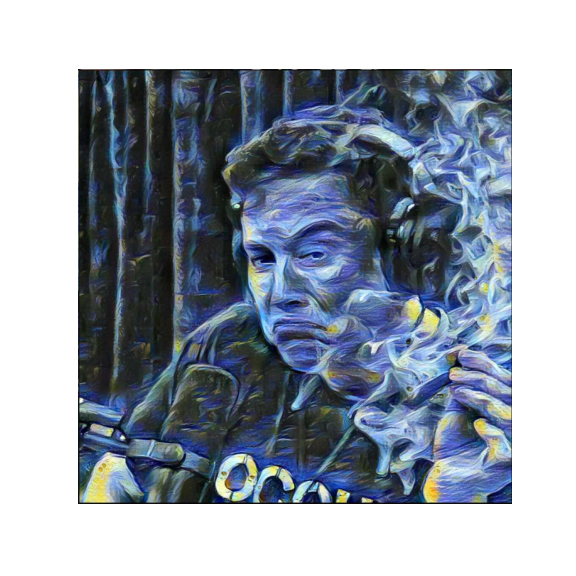
\includegraphics[scale=0.38]{assets/elon_canaGAN.png}
    \vspace{-50pt}
    \caption{Elon Musk}
  \end{minipage}
  \hfill
  \begin{minipage}[c]{0.49\linewidth}
    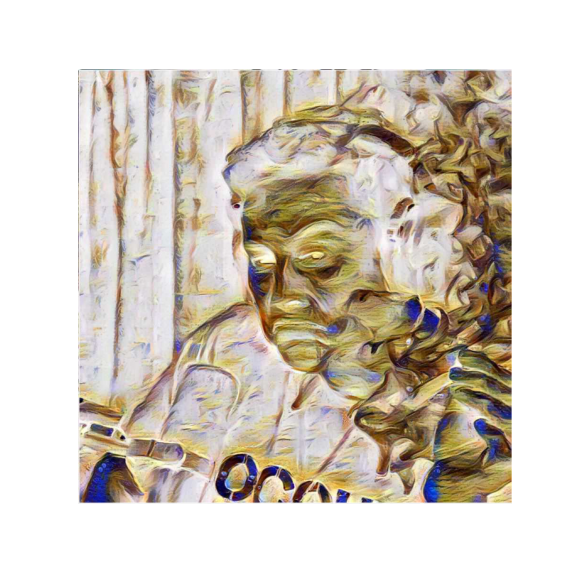
\includegraphics[scale=0.38]{assets/elon_inverted.png}
    \vspace{-50pt}
    \caption{Inverted filter}
  \end{minipage}
  \vspace{-20pt}
  \begin{minipage}[l]{0.49\linewidth}
    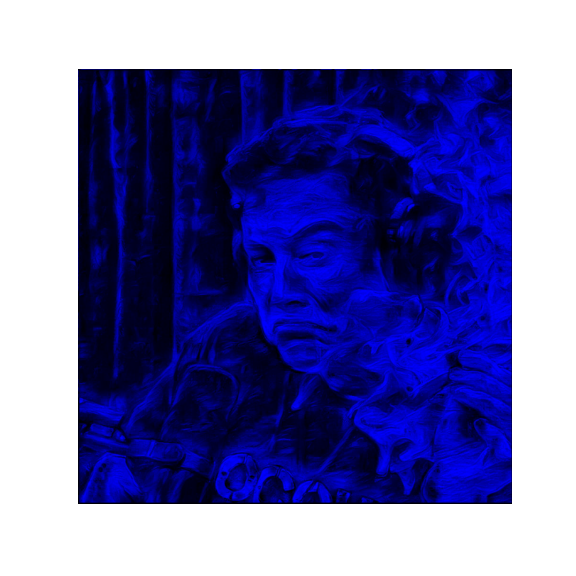
\includegraphics[scale=0.38]{assets/elon_blue.png}
    \vspace{-50pt}
    \caption{Blue filter}
  \end{minipage}
  \hfill
  \begin{minipage}[c]{0.49\linewidth}
    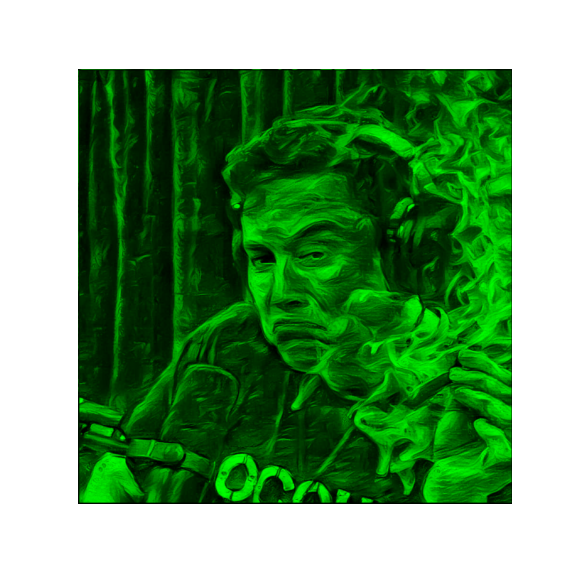
\includegraphics[scale=0.38]{assets/elon_green.png}
    \vspace{-50pt}
    \caption{Green filter}
  \end{minipage}
  \vspace{-20pt}
  \begin{minipage}[l]{0.49\linewidth}
    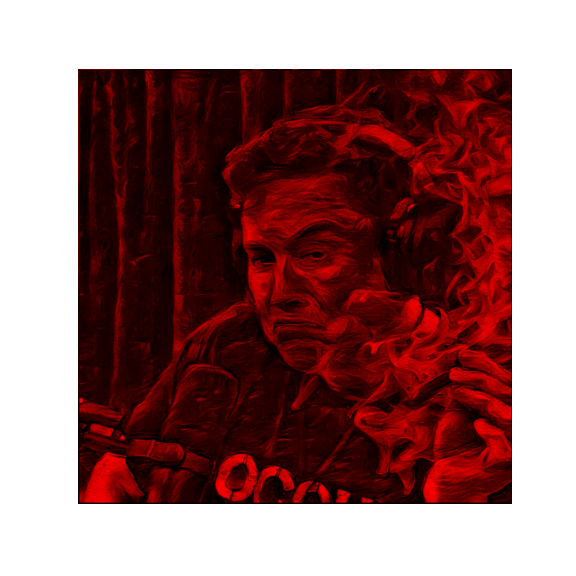
\includegraphics[scale=0.38]{assets/elon_red.png}
    \vspace{-50pt}
    \caption{Red filter}
  \end{minipage}
  \hfill
  \begin{minipage}[c]{0.49\linewidth}
    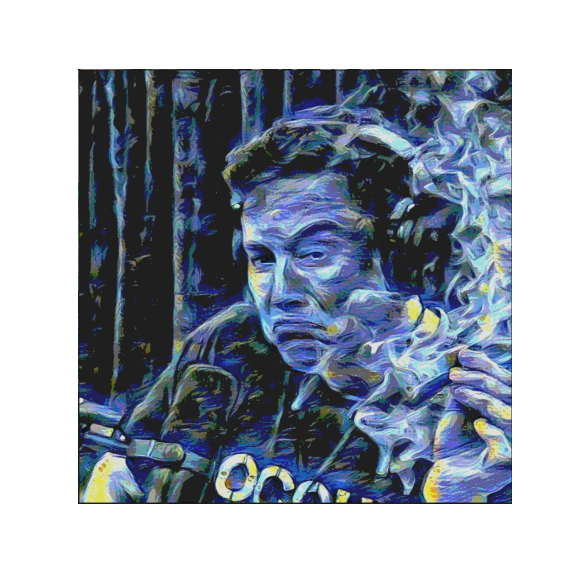
\includegraphics[scale=0.38]{assets/elon_celluloid.png}
    \vspace{-50pt}
    \caption{Celluloid filter}
  \end{minipage}
  
\end{figure}

\info{
The first image is a stylization of Elon Musk that has been generated using a style transfer algorithm implemented in our lab.
You can see the code in 42AI repository \href{https://github.com/42-AI/StyleTransferMirror}{StyleTransferMirror}}
